\documentclass[../main.tex]{subfiles}
\begin{document}
	
	\section{Lista 2}


\begin{exercicio}{1}
	Calcule o comprimento de arco das seguintes curvas:
	
	\begin{enumerate}[label=\alph*)]
		\item $\alpha(t) = (3\cosh{2t}, 3\sinh{2t},6t)$, $t\in [0,\pi]$.
		\item Catenária: $\gamma(t)=(t,\cosh(t))$, a partir do ponto $(0,1)$.
	\end{enumerate}
\end{exercicio}

\begin{solucao}
	\begin{definicao}[Comprimento de arco]
		O comprimento de arco de uma curva regular do ponto $\alpha(a)$ até $\alpha(b)$ é dado por:
		\[
		\mathcal{L}_a^b(\alpha)=\int_a^b \|\alpha'(t)\|\,dt
		\]
	\end{definicao}
	
	Assim, para calcular o comprimento de arco das curvas, basta derivá-la, tirar sua norma e aplicar a integral.
	
	\begin{enumerate}[label=\alph*)]
		\item $\alpha'(t)=((3\cosh{2t})',(3\sinh{2t})',(6t)')=(3\cdot 2\sinh{2t},3\cdot 2\cosh{2t}, 6)$
		
		$\Rightarrow \|\alpha'(t)\|=\sqrt{(6\sinh{2t})^2+(6\cosh{2t})^2+6^2}=6\cdot \sqrt{\sinh^2(2t)+\cosh^2(2t)+1}$
		
		$\Rightarrow \|\alpha'(t)\|=6\cdot \sqrt{\sinh^2(2t)+\cosh^2(2t)-\sinh^2(2t)+\cosh^2(2t)}$
		
		$\Rightarrow \|\alpha'(t)\|=6\sqrt{2}\cdot \sqrt{\cosh^2(2t)}=6\sqrt{2}\cdot \cosh(2t)$
		
		$\Rightarrow \int_a^b \|\alpha'(t)\|\,dt=\int_a^b 6\sqrt{2}\cdot \cosh(2t)\,dt$
		
		$\Rightarrow \mathcal{L}_0^\pi(\alpha)=6\sqrt{2}\cdot \int_0^{2\pi} \cosh{u}\, du=3\sqrt{2}\cdot (\sinh(2\pi)-\sinh(0))=3\sqrt{2}\cdot (\sinh(2\pi)-0)$
		
		$\Rightarrow \mathcal{L}_0^\pi(\alpha)=3\sqrt{2}\cdot \sinh(2\pi)$
		
		\item No ponto $(0,1)$, temos:
		$(0,1)=(t,\cosh(t))\Rightarrow t=0$
		
		Com isso, podemos calcular o comprimento de arco de $t=0$ até um certo ponto $t=b$.
		
		$\gamma'(t)=(t', (\cosh(t))')=(1,\sinh(t))$
		
		$\Rightarrow \|\gamma'(t)\|=\sqrt{1+\sin^2(t)}=\sqrt{\cosh^2(t)}=\cosh(t)$
		
		$\Rightarrow \mathcal{L}_0^b(\gamma)=\int_0^b \cosh(t)\,dt=\sinh(b)-\sinh(0)=\sinh(b)$
		
	\end{enumerate}
\end{solucao}

\begin{exercicio}{3}
	Mudanças de parâmetro:
	
	\begin{enumerate}[label=\alph*)]
		\item Demonstrar que $s(\theta)=\frac{\theta^2}{\theta^2+1}$ é uma mudança de parâmetro diferenciável que tranforma o intervalo $(0,\infty)$ no intervalo $(0, 1)$.
		\item Mostrar que a função $\lambda:(-1, 1)\rightarrow(-\infty,+\infty)$, definida por $\lambda(t)\coloneqq \tan(\frac{\pi t}{2})$ é uma mudança de parâmetro.
		\item  Provar que qualquer curva pode ser reparametrizada de forma tal que o domínio da reparametrização seja um intervalo de extremos $0$ e $1$.
	\end{enumerate}
\end{exercicio}

\begin{solucao}
	\begin{definicao}[Mudança de parâmetro] 
		Duas funções vetoriais de uma variável real $f(t) : I\subset \mathbb{R}\rightarrow \mathbb{R}^n$ e $g(s) : I_{0} \subset \mathbb{R} \rightarrow \mathbb{R}^n$ se dizem equivalentes quando possuem o mesmo gráfico (traço).
		
		Uma função real bijetora $u(t) : I_{0}\rightarrow I$, derivável, e que a derivada não se anula, tal que
		$$g(t) = f(u(t))$$
		define uma mudança de parâmetro.
	\end{definicao}
	
	\begin{enumerate}[label=\alph*)]
		\item Para demonstrar que $s(\theta)$ é uma mudança de parâmtro diferenciável tal que $s:(0,\infty)\rightarrow(0,1)$, queremos provar que:
		
		\begin{enumerate}[label=\roman*)]
			\item $s$ é derivável em todo ponto em $(0,\infty)$, tal que ela nunca se anula;
			\item $s$ é bijetiva;
			\item $s$ leva $(0,\infty)\rightarrow(0,1)$ 
		\end{enumerate}
		
		\begin{proof}[Prova de i)]
			
			\begin{teorema}[Teorema 4.1; Calculus; Tom M. Apostol; p. 164]
				Sejam $f$ e $g$ duas funções definidas em um intervalo comum. Se cada ponto onde $f$ e $g$ têm uma derivada, o mesmo é verdadeiro para [...] o quoiente $f/g$. (Para $f/g$ nós precisamos da condição extra de que $g$ é diferente de zero nesse ponto.) [...].
			\end{teorema}
			
			Por esse teorema, temos que, como $f(\theta)=\theta^2$ e $g(\theta)=\theta^2+1$ são polinômios do segundo grau, eles são diferenciáveis em $(0,\infty)$. Em particular, também temos que $g(\theta)\neq 0$, $\forall \theta\in \mathbb{R}$.
			
			$$\theta^2+1=0\Rightarrow \theta=\sqrt{-1}\Rightarrow \theta\notin \mathbb{R}$$
			
			Logo, $s$ é derivável em todo o ponto em $(0,\infty)$.
			
			Além disso, note que
			
			$s'(\theta)=\frac{2\theta(\theta^2+1)-\theta^2(2\theta)}{(\theta^2+1)^2}=\frac{2\theta}{(\theta^2+1)^2}$
			
			$s'(\theta)=0\Leftrightarrow 2\theta=0\Leftrightarrow \theta=0$
			
			Assim $s'(\theta)\neq0$, $\forall \theta \in (0,\infty)$.
			
		\end{proof}
		
		\begin{proof}[Prova de ii) e iii)]
			
			Por definição, $s$ é bijetiva se, e somente se, $s$ é injetiva e sobrejetiva.
			
			Tome dois números arbitrários $x,y\in\mathbb{R}$, tal que $x\neq y$. Sem perda de generalidade, assuma que $x>y$.
			
			$x>y\Rightarrow x^2+1>y^2+1\Rightarrow -\frac{1}{x^2+1}>\frac{1}{y^2+1}$
			
			$\Rightarrow 1-\frac{1}{x^2+1}>1-\frac{1}{y^2+1}\Rightarrow \frac{x^2}{x^2+1}>\frac{y^2}{y^2+1}\Rightarrow s(x)>s(y)$
			
			$\therefore x>y\Rightarrow s(x)>s(y)$
			
			Assim, temos $s$ estritamente crescente e, portanto, injetiva.
			
			Além disso, podemos tomar o limite da função nos extremos do domínio e verificar sua sobrejetividade, devido ao fato de $s$ ser contínua, bem como a propriedade iii).
			
			$\lim_{\theta \to 0^{+}}\frac{\theta^2}{\theta^2+1}=\frac{\lim_{\theta \to 0^{+}}\theta^2}{\lim_{\theta \to 0^{+}}\theta^2+1}=\frac{0}{1}=0$
			
			$\lim_{\theta \to \infty}\frac{\theta^2}{\theta^2+1}=\lim_{\theta \to \infty}\frac{2\theta}{2\theta}=\lim_{\theta \to \infty}1=1$
			
			Pela propriedade estritamente crescente de $s$, temos que a imagem de $s$ é $(0,1)$, que é igual ao contradomínio e, portanto, verifica a sobrejetividade de $s$. Em outras palavras, temos que $s$ leva $(0,\infty)\rightarrow(0,1)$.
			
		\end{proof}
		
		Portanto, demonstramos que $s$ é uma mudança de parâmetro diferenciável, que transforma o intervalo $(0,\infty)$ no intervalo $(0,1)$.
		
		\item Para demonstrar que $\lambda$ é uma mudança de parâmtro, queremos provar que:
		
		\begin{enumerate}[label=\roman*)]
			\item $\lambda$ é derivável em todo ponto em $(-1,1)$;
			\item $\lambda'(t)\neq 0$, $\forall t\in (-1,1)$;
			\item $\lambda$ é bijetiva.
		\end{enumerate}
		
		\begin{proof}[Prova de i)]
			Podemos escrever $\lambda$ como $\lambda(t)=f(g(t))$, tal que $g(t)=\frac{\pi t}{2}$ e $f(t)=\tan(t)$. Note que $g$ é derivável e, por ser um polinômio de primeiro grau crescente, ao considerar o domínio $(-1,1)$, temos que sua imagem é $(g(-1), g(1))=(-\frac{\pi}{2}, \frac{\pi}{2})$. 
			Por definição, a função tangente tem como domínio $(-\frac{\pi}{2}, \frac{\pi}{2})$ e como imagem $(-\infty, +\infty)$, e também é derivável.
			Assim, pela regra da cadeia, temos que $\lambda$ é derivável em todo ponto em $(-1,1)$.
		\end{proof}
		
		\begin{proof}[Prova de ii)]
			Pela regra da cadeia, temos que
			$\lambda'(t)=(\tan(\frac{\pi t}{2}))'=\frac{\pi}{2}\cdot \sec(\frac{\pi t}{2})$. Note que a função secante, por definição, é o inverso do cosseno e, portanto, nunca se iguala a zero. dessa forma, $\lambda'(t)\neq 0$, $\forall t \in (-1,1)$.
		\end{proof}
		
		\begin{proof}[Prova de iii)]
			Note que, pelos argumentos i) e ii), a imagem de $\lambda$ é $\mathbb{R}$, fazendo dela sobrejetiva; e $\lambda'(t)\neq 0$ em todo o domínio, ou seja, $\lambda$ é monótona e, portanto, injetiva. Logo, temos $\lambda$ bijetiva.
		\end{proof}
		\item  \begin{proof}
			Vamos analisar três casos:
			
			\begin{enumerate}[label=\textbf{Caso \arabic*:}]
				\item Seja $I_0$ um intervalo fechado ou aberto, com extremos $a$ e $b$, tal que $a\neq b$, que é o domínio de uma parametrização $f$. Podemos definir uma função de reparametrização $\varphi$, com domínio de extremos $0$ e $1$, tal que
				$$\varphi(s)=a+(b-a)s$$
				Note que $\varphi(0)=a$ e $\varphi(1)=b$. Além disso, por ser uma função do primeiro grau, ela é bijetiva, diferenciável e sua derivada é não nula.
				Assim, a nova parametrização $g$ pode ser definida como $g(t)\coloneq f(\varphi(t))$, onde o domínio de $g$ é um intervalo de extremos $0$ e $1$ e, ao mesmo tempo, descreve a mesma curva que $f$.
				\item Seja  $I_0=(a,\infty)$ o domínio de uma parametrização $f$. Pelo item a), a função $s$ é bijetiva e, portanto, possui uma função inversa $s^{-1}:(0,1)\rightarrow(0,\infty)$. Com isso, podemos definir uma nova parametrização $g$, sendo $s^{-1}$ a função de reparemtrização, tal que $g(t)\coloneq f(s^{-1}(t+a))$ possui domínio de extremos $0$ e $1$. Para $I_0=(-\infty,b)$, basta definir $a\coloneq -b$, e uma função de reparametrização $r$, tal que $r(t)\coloneq -s^{-1}(t)$.
				\item Seja  $I_0=(-\infty,+\infty)$ o domínio de uma parametrização $f$. Dada a funçãp $\lambda$ do item b), defina $\lambda_1(t)\coloneq \lambda(2t-1)$. Note que o domínio de $\lambda_1$ pode ser definido por $(\lambda_1(-1),\lambda_1(1))=(\frac{-1+1}{2},\frac{1+1}{2})=(0,1)$, e sua imagem é a mesma de $\lambda$, $(-\infty,+\infty)$. Com isso, podemos definir uma nova parametrização $g$, sendo $\lambda_1$ a função de reparametrização, tal que $g(t)\coloneq f(\lambda_1(t))$ possui domínio de extremos $0$ e $1$.
			\end{enumerate}
			
		\end{proof}
	\end{enumerate}
\end{solucao}


\begin{exercicio}{6}
	Reproduza, no ambiente computacional de sua preferência, os vetores $\alpha'$ e $\alpha''$ para uma curva $\alpha$ de sua preferência com duas parametrizações distintas, sendo uma a parametrização por comprimento de arco. Observe que para a parametrização por comprimento de arco o ângulo entre $\alpha'$ e $\alpha''$ é um ângulo reto, o que não ocorre em uma parametrização arbitrária.
\end{exercicio}

\begin{solucao}
	A curva escolhida foi a hélice circular, dada por $\alpha(t)=(\cos(t),\sin(t), t)$.
	
	Note que
	\[
	\alpha'(t)=(-\sin(t),\cos(t),1)\Rightarrow\|\alpha'(t)\|=\sqrt{\sin^2(t)+\cos^2(t)+1}=\sqrt{2}
	\]
	
	Logo, essa parametrização arbitrária da hélice circular não é unit-speed. Para parametrizá-la com um novo $\beta$, podemos definir uma função de reparametrização $\varphi(t)=\frac{t}{\sqrt{2}}$. Assim, temos
	\[
	\beta(t)=\alpha(\varphi(t))=(\cos(\tfrac{t}{\sqrt{2}}), \sin(\tfrac{t}{\sqrt{2}}), \tfrac{t}{\sqrt{2}})
	\]
	\[
	\Rightarrow \beta'(t)=(-\tfrac{1}{\sqrt{2}}\sin(\tfrac{t}{\sqrt{2}}), \tfrac{1}{\sqrt{2}}\cos(\tfrac{t}{\sqrt{2}}), \tfrac{1}{\sqrt{2}})
	\]
	\[
	\Rightarrow \|\beta'(t)\|=\sqrt{\tfrac{1}{2}\sin^2(t)+\tfrac{1}{2}\cos^2(t)+\tfrac{1}{2}}=1
	\]
	
	Assim, temos escolhidas duas parametrizações distintas, $\alpha$ e $\beta$, tal que uma delas ($\beta$) é parametrizada por comprimento de arco. As figuras 1 e 2 mostram essas parametrizações plotadas.
	
	\begin{center}
		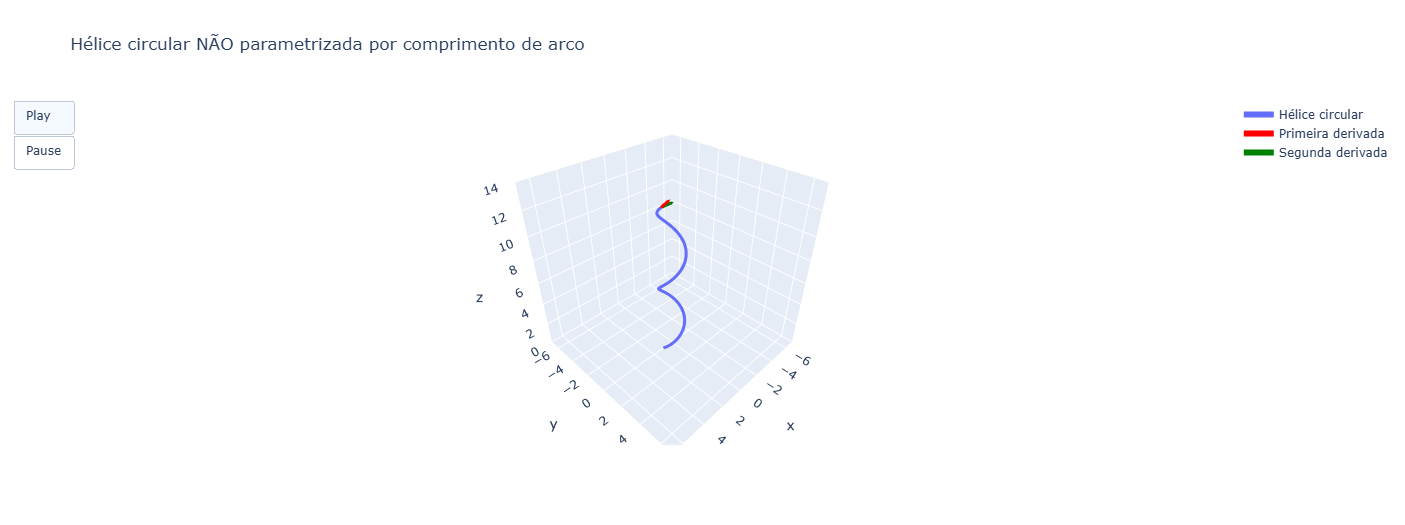
\includegraphics[width=0.5\textwidth]{imagens/lista02/picture_lista02_q06_item01.png}
		\captionof{figure}{Hélice não parametrizada}
	\end{center}
	
	\begin{center}
		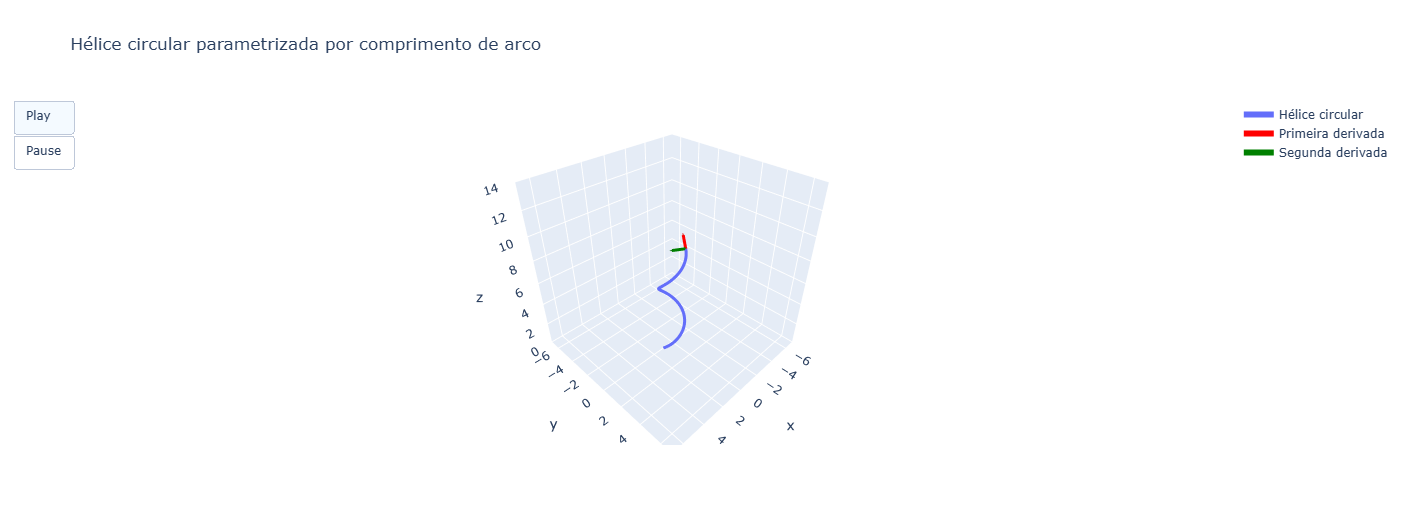
\includegraphics[width=0.5\textwidth]{imagens/lista02/picture_lista02_q06_item02.png}
		\captionof{figure}{Hélice parametrizada}
	\end{center}
\end{solucao}

\begin{exercicio}{7}
	Verifique a regularidade e calcule o comprimento de arco e a curvatura
	das seguintes curvas, quando possível:
	
	\begin{itemize}
		\item (retas) $\alpha(t)=(a + ct, b + dt)$, $t\in \mathbb{R}$;
		\item $\alpha(t)=(t, t^4)$, $t\in \mathbb{R}$;
		\item (círculos) $\alpha(s)=(a + r\cdot \cos(\frac{s}{r}), b+r\cdot \sin(\frac{s}{r}))$, $s\in \mathbb{R}$, $r>0$;
		\item (cardióide) $\alpha(t)=(\cos(t)\cdot (2\cos(t) - 1), \sin(t)\cdot (2\cos(t) -1))$, $t\in \mathbb{R}$;
		\item (catenária) $\alpha(t)=(t, \cosh(t))$, $t\in \mathbb{R}$.
	\end{itemize}
\end{exercicio}

\begin{solucao}
	\begin{itemize}
		\item \textbf{Retas}
		\begin{itemize}
			\item \textbf{Regularidade:} como $\alpha(t)=(a+ct,b+dt)\Rightarrow \alpha'(t)=(c,d)$, e $c,d\neq 0\Rightarrow \alpha'(t)\neq (0,0)$, então temos uma curva regular, pois a derviada não se anula.
			\item \textbf{Comprimento de arco:}  $\mathcal{L}_{t_1}^{t_2}(\alpha)=\int_{t_1}^{t_2} \sqrt{c^2+d^2}\, dt=\sqrt{c^2+d^2}\cdot (t_2-t_1)$
			\item \textbf{Curvatura:} note que $\alpha''(t)=(0,0)$. Assim, $k_\alpha(t)=\frac{\det\big[(c,d), (0,0)\big]}{\|(c,d)\|^3}=0$
		\end{itemize}
		\item \textbf{$(t,t^4)$}
		\begin{itemize}
			\item \textbf{Regularidade:} $\alpha(t)=(t,t^4)\Rightarrow \alpha'(t)=(1,4t^3)\Rightarrow \alpha'(t)\neq(0,0)$,$\forall t\in \mathbb{R}\Rightarrow \alpha$ é regular.
			\item \textbf{Comprimento de arco:}  $\mathcal{L}_{t_1}^{t_2}(\alpha)=\int_{t_1}^{t_2} \sqrt{1^2+(4t^3)^2}\, dt=\int_{t_1}^{t_2} \sqrt{1+16t^6}\, dt$
			\item \textbf{Curvatura:} note que $\alpha''(t)=(0,12t^2)$. Assim,
			
			$k_\alpha(t)=\frac{\det\big[(1,4t^3), (0,12t^2)\big]}{\|(1,4t^3)\|^3}=\frac{12t^2}{(1+16t^6)^{\frac{3}{2}}}$
		\end{itemize}
		\item \textbf{Círculos}
		\begin{itemize}
			\item \textbf{Regularidade:} $\alpha(s)=(a+r\cdot \cos(\frac{s}{r}),b+r\cdot \sin(\frac{s}{r}))\Rightarrow \alpha'(t)=(-\sin(\frac{s}{r}),\cos(\frac{s}{r}))$ 
			
			Note que $-\sin(\theta)=\cos(\theta)\Leftrightarrow\theta=\arctan(-1)$. Como $\arctan(-1)\neq 0$, temos que
			
			$\alpha'(t)\neq(0,0)$,$\forall t\in \mathbb{R}\Rightarrow \alpha$ é regular.
			\item \textbf{Comprimento de arco:}  $\mathcal{L}_{t_1}^{t_2}(\alpha)=\int_{t_1}^{t_2} \sqrt{(-\sin(\frac{s}{r}))^2+(\cos(\frac{s}{r}))^2}\, dt=\int_{t_1}^{t_2} \sqrt{1}\, dt=t_2-t_1$
			\item \textbf{Curvatura:} note que $\alpha''(t)=(-\frac{1}{r}\cdot \cos(\frac{s}{r}),-\frac{1}{r}\cdot \sin(\frac{s}{r}))$. Assim,
			
			$k_\alpha(t)=\frac{\det\big[(-\sin(\frac{s}{r}),\cos(\frac{s}{r})), (-\frac{1}{r}\cdot \cos(\frac{s}{r}),-\frac{1}{r}\cdot \sin(\frac{s}{r}))\big]}{\|(-\sin(\frac{s}{r}),\cos(\frac{s}{r}))\|^3}=\frac{\frac{1}{r}\cdot \sin^2(\frac{s}{r})+\frac{1}{r}\cdot \cos^2(\frac{s}{r})}{1^3}=\frac{1}{r}$
			
			Outra forma de pensar é que, como $\|\alpha'(t)\|=1$, a curva é unit-speed e temos
			
			$|k_\alpha(t)|=\|\alpha''(t)\|=\frac{1}{r}$
		\end{itemize}
		\item \textbf{Cardióide}
		\begin{itemize}
			\item \textbf{Regularidade:} $\alpha(t)=(\cos(t)\cdot (2\cos(t)-1),\sin(t)\cdot (2\cos(t)-1))$
			
			$\Rightarrow \alpha'(t)=(-\sin(t)(2\cos(t)-1)+\cos(t)\cdot2(-sin(t)),\cos(t)(2\cos(t)-1)+\sin(t)\cdot 2(-sin(t)))$.
			
			$\Rightarrow \alpha'(t)=(\sin(t)-2\sin(2t), 2\cos(2t)-\cos(t))$
			
			$\Rightarrow \|\alpha'(t)\|^2=\sin^2(t)-4\sin(t)\sin(2t)+4\sin^2(2t)+4\cos^2(2t)-4\cos(2t)\cos(t)+\cos^2(t)$
			
			$\Rightarrow \|\alpha'(t)\|^2=1+4-4(\sin(t)\sin(2t)+\cos(t)\cos(2t))=5-4(\cos(2t-t))$
			
			$\Rightarrow \|\alpha'(t)\|^2=5-4\cos(t)\Rightarrow\|\alpha'(t)\|^2\geq5-4=1$, $\forall t \in \mathbb{R}$
			
			$\Rightarrow \|\alpha'(t)\|\neq 0$, $\forall t \in \mathbb{R}\Rightarrow \alpha$ é regular.
			\item \textbf{Comprimento de arco:}  $\mathcal{L}_{t_1}^{t_2}(\alpha)=\int_{t_1}^{t_2} \sqrt{\|\alpha'(t)\|^2}\, dt=\int_{t_1}^{t_2} \sqrt{5-4\cos(t)}\, dt$
			\item \textbf{Curvatura:}
			
			$\alpha''(t)=(\alpha'(t))'=(\cos(t)-4\cos(2t), \sin(t)- 4\sin(2t))$
			
			{\footnotesize
				$\Rightarrow k_\alpha(t)=
				\tfrac{
					\det\big[(\sin(t)-2\sin(2t), 2\cos(2t)-\cos(t)), (\cos(t)-4\cos(2t), \sin(t)-4\sin(2t))\big]
				}{
					\|(\sin(t)-2\sin(2t), 2\cos(2t)-\cos(t))\|^3
				}$
			}
			
			{\small
				$\Rightarrow k_\alpha(t)=\tfrac{\sin^2(t)-6\sin(t)\sin(2t)+8\sin^2(2t)+\cos^2(t)-6\cos(t)\cos(2t)+8\cos^2(2t)}{(5-4\cos(t))^{\frac{3}{2}}}$
				
				$\Rightarrow k_\alpha(t)=\frac{1+8-6(\sin(t)\sin(2t)+\cos(t)\cos(2t))}{(5-4\cos(t))^{\frac{3}{2}}}$
			}
			
			$\Rightarrow k_\alpha(t)=\frac{9-6\cos(t)}{(5-4\cos(t))^{\frac{3}{2}}}$
		\end{itemize}
		\item \textbf{Catenária}
		\begin{itemize}
			\item \textbf{Regularidade:} $\alpha(t)=(t,\cosh(t))\Rightarrow \alpha'(t)=(1,\sinh(t))\Rightarrow \alpha'(t)\neq(0,0)$,$\forall t\in \mathbb{R}\Rightarrow \alpha$ é regular.
			\item \textbf{Comprimento de arco:}  $\mathcal{L}_{t_1}^{t_2}(\alpha)=\int_{t_1}^{t_2} \sqrt{1^2+(\sinh(t))^2}\, dt=\int_{t_1}^{t_2} \sqrt{\cosh^2(t)}\, dt$
			
			$\Rightarrow \mathcal{L}_{t_1}^{t_2}(\alpha)=\sinh(t_2)-\sinh(t_1)$
			\item \textbf{Curvatura:} note que $\alpha''(t)=(0,\cosh(t))$. Assim,
			
			$k_\alpha(t)=\frac{\det\big[(1,\sinh(t)), (0,\cosh(t))\big]}{\|(1,\sinh(t))\|^3}=\frac{\cosh(t)}{(\cosh^2(t))^{\frac{3}{2}}}$
			
			$\Rightarrow k_\alpha(t)=\frac{\cosh(t)}{\cosh^3(t)}=(\cosh(t))^{-2}=sinh^2(t)$
		\end{itemize}
	\end{itemize}
\end{solucao}

\begin{exercicio}{8}
	Considere a elipse $\beta(t)=(a\cdot \cos(t), b\cdot sin(t))$, $t\in \mathbb{R}$, onde $a > 0$, $b > 0$ e $a\neq b$. Obtenha os valores de $t$ onde a curvatura de $\beta$ é máxima e mínima.
\end{exercicio}

\begin{solucao}
	Derivando $\beta$, temos
	\begin{itemize}
		\item $\beta'(t)=(-a\cdot \sin(t), b\cdot \cos(t))$
		\item $\beta''(t)=(-a\cdot \cos(t), -b\cdot \sin(t))$
	\end{itemize}
	
	Pela definição de curvatura, temos que
	{\footnotesize
		\[
		k_{\beta}(t) = \frac{\det(\beta'(t),\beta''(t))}{\|\beta'(t)\|^3} = \frac{ab\sin^2(t) + ab\cos^2(t)}{(a^2\sin^2(t)+b^2\cos^2(t))^{3/2}} = \frac{ab}{(a^2\sin^2(t)+b^2\cos^2(t))^{3/2}}
		\]
	}
	
	Para obter os máximos e mínimos dessa função, basta derivá-la e encontrar $t$, tal que $k_\beta'(t)=0$:
	
	{\footnotesize
		\[
		k'_{\beta}(t) = ab \cdot \Big(-\tfrac{3}{2}\Big)
		\big(a^2\sin^2(t) + b^2\cos^2(t)\big)^{-5/2}
		\cdot \big(2a^2\sin(t)\cos(t) - 2b^2\cos(t)\sin(t)\big)=0
		\]
		\[
		\Rightarrow 2(a^2-b^2)\sin(t)\cos(t)=0\Rightarrow \sin(2t)=0\Rightarrow t=\frac{n\pi}{2}(n\in \mathbb{Z)}
		\]
	}
	
	A última implicação ocorre porque $a > 0$, $b > 0$ e $a\neq b$.
	
	Derivando uma segunda vez, temos
	
	\[
	k_\beta'(t)=-\tfrac{3ab}{2}
	\big(a^2\sin^2(t) + b^2\cos^2(t)\big)^{-5/2}
	\cdot (a^2-b^2)\sin(2t)
	\]
	
	\[
	\Rightarrow k_\beta''(t)=-\frac{3ab(a^2-b^2)}{2}\bigg(2\cos(2t)\big(a^2\sin^2(t) + b^2\cos^2(t)\big)^{-5/2}
	\]
	\[
	+\sin(2t)\big(\tfrac{-5}{2}\big)\big(a^2\sin^2(t)+b^2\cos^2(t)\big)^{-7/2}(a^2-b^2)\sin(2t)\bigg)
	\]
	
	Aplicando para $t=\frac{n\pi}{2}$, quando $n$ é ímpar,
	
	\[
	k_\beta''(\tfrac{n\pi}{2})=-\frac{3ab(a^2-b^2)}{2}\bigg(2\cos(n\pi)\big(a^2\sin^2(\tfrac{n\pi}{2}) + b^2\cos^2(\tfrac{n\pi}{2})\big)^{-5/2}
	\]
	\[
	+\sin(n\pi)\big(\tfrac{-5}{2}\big)\big(a^2\sin^2(\tfrac{n\pi}{2})+b^2\cos^2(\tfrac{n\pi}{2})\big)^{-7/2}(a^2-b^2)\sin(n\pi)\bigg)
	\]
	
	\[
	\Rightarrow k_\beta''(\tfrac{n\pi}{2})=-\frac{3ab(a^2-b^2)}{2}\bigg(2(-1)^n\big(a^2(-1)^{2n} + b^2\cdot 0\big)^{-5/2}
	\]
	\[
	+0\cdot \big(\tfrac{-5}{2}\big)\big(a^2(-1)^{2n}+b^2\cdot 0\big)^{-7/2}(a^2-b^2)\cdot 0\bigg)
	\]
	
	\[
	\Rightarrow k_\beta''(\tfrac{n\pi}{2})=-\frac{3ab(a^2-b^2)}{2}\bigg(2(-1)^n\big(a^2)^{-5/2}\bigg)
	\]
	
	\[
	\Rightarrow k_\beta''(\tfrac{n\pi}{2})=-3ab(a^2-b^2)(-1)^na^{-5}=\frac{3b(a^2-b^2)}{a^4}
	\]
	
	Para $n$ par, temos
	
	\[
	k_\beta''(\tfrac{n\pi}{2})=-\frac{3ab(a^2-b^2)}{2}\bigg(2\cos(n\pi)\big(a^2\sin^2(\tfrac{n\pi}{2}) + b^2\cos^2(\tfrac{n\pi}{2})\big)^{-5/2}
	\]
	\[
	+\sin(n\pi)\big(\tfrac{-5}{2}\big)\big(a^2\sin^2(\tfrac{n\pi}{2})+b^2\cos^2(\tfrac{n\pi}{2})\big)^{-7/2}(a^2-b^2)\sin(n\pi)\bigg)
	\]
	
	\[
	\Rightarrow k_\beta''(\tfrac{n\pi}{2})=-\frac{3ab(a^2-b^2)}{2}\bigg(2(-1)^n\big(a^2\cdot 0 + b^2(-1)^{2n}\big)^{-5/2}
	\]
	\[
	+0\cdot \big(\frac{-5}{2}\big)\big(a^2\cdot 0+b^2(-1)^{2n}\big)^{-7/2}(a^2-b^2)\cdot 0\bigg)
	\]
	
	\[
	\Rightarrow k_\beta''(\tfrac{n\pi}{2})=-\frac{3ab(a^2-b^2)}{2}\bigg(2(-1)^n\big(b^2)^{-5/2}\bigg)
	\]
	
	\[
	\Rightarrow k_\beta''(\tfrac{n\pi}{2})=-3ab(a^2-b^2)(-1)^nb^{-5}=\frac{-3a(a^2-b^2)}{b^4}
	\]
	
	Caso $a>b\Rightarrow a^2-b^2>0$, temos que
	\begin{itemize}
		\item Para $n$ ímpar, $k_\beta''(\tfrac{n\pi}{2})>0\Rightarrow t=\tfrac{n\pi}{2}$ é ponto de mínimo.
		\item Para $n$ par, $k_\beta''(\tfrac{n\pi}{2})<0\Rightarrow t=\tfrac{n\pi}{2}$ é ponto de máximo.
	\end{itemize}
	
	Caso $a<b\Rightarrow a^2-b^2<0$, temos que
	\begin{itemize}
		\item Para $n$ ímpar, $k_\beta''(\tfrac{n\pi}{2})<0\Rightarrow t=\tfrac{n\pi}{2}$ é ponto de máximo.
		\item Para $n$ par, $k_\beta''(\tfrac{n\pi}{2})>0\Rightarrow t=\tfrac{n\pi}{2}$ é ponto de mínimo.
	\end{itemize}
\end{solucao}

\begin{exercicio}{9}
	Reproduza, no ambiente computacional de sua preferência, a representação gráfica da \textit{Tangente Indicatrix}, conforme exemplificado no arquivo .ggb apresentado em aula. Teste com a curva de sua preferência.
\end{exercicio}

\begin{solucao}
	A animação utilizou a curva $\alpha(t)=(t,t^2,t^3)$, em que a tangente indicatrix, que está plotada à esquerda, apresenta a reta tangente $\alpha'(t)$. À direita está a curva e as tangentes propriamente ditas. Segue na figura 3 uma das imagens da animação.
	
	\begin{center}
		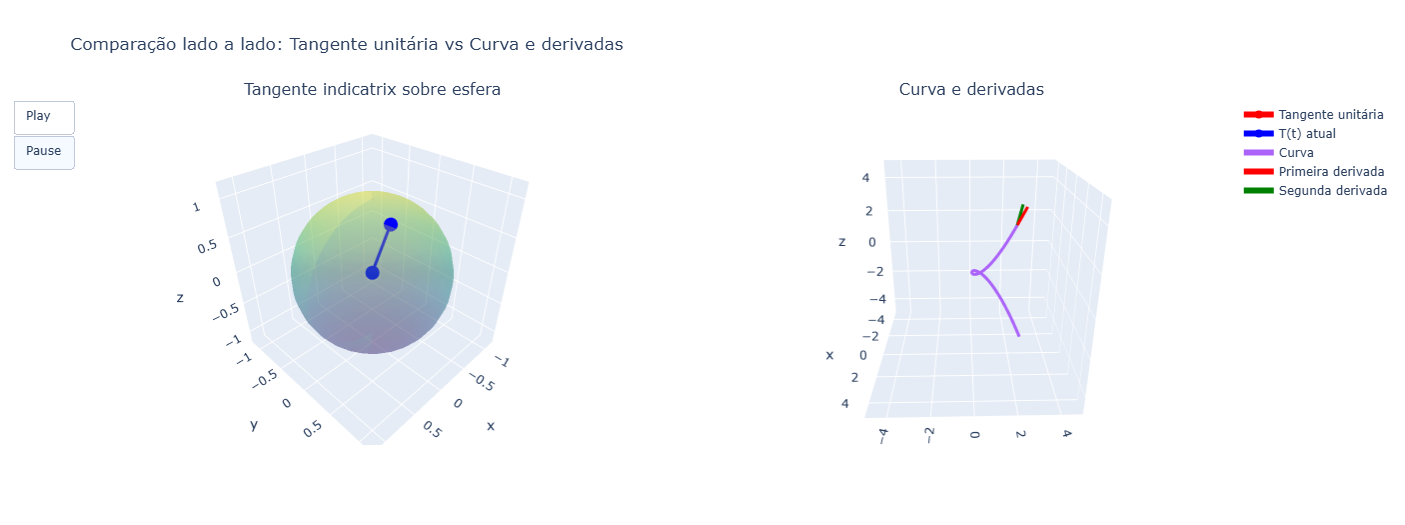
\includegraphics[width=0.5\textwidth]{imagens/lista02/picture_lista02_q09.png}
		\captionof{figure}{Tangente Indicatrix}
	\end{center}
\end{solucao}

\begin{exercicio}{13}
	Em ambiente computacional, desenhe as seguintes curvas e produza
	uma animação do Triedro de Frenet de cada curva:
	\begin{enumerate}[label=\alph*)]
		\item $\alpha(t)=(4\cdot \cos(t), 5-5\cdot \sin(t),-3\cdot \cos(t))$, $t\in \mathbb{R}$
		\item $\beta(t)=(1-\cos(t), \sin(t), t)$, $t\in \mathbb{R}$
	\end{enumerate}
\end{exercicio}

\begin{solucao}
	Segue nas figuras 4 e 5 uma imagem de cada animação dos itens a) e b), respectivamente.
	
	\begin{center}
		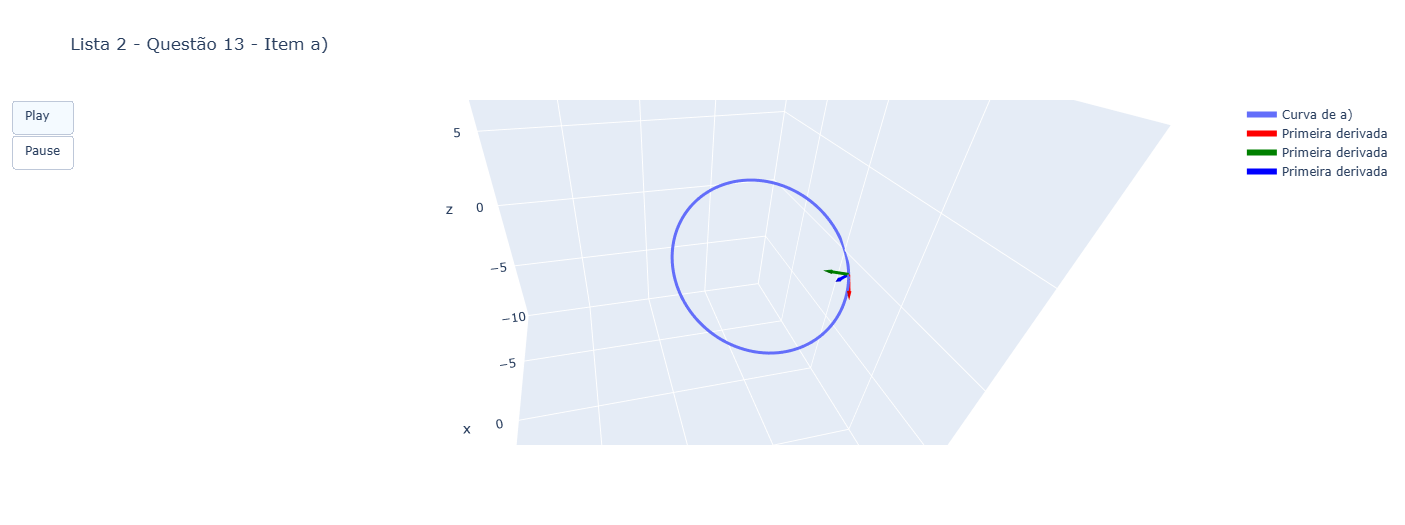
\includegraphics[width=0.5\textwidth]{imagens/lista02/picture_lista02_q13_item01.png}
		\captionof{figure}{Questão 13 - Item a)}
	\end{center}
	\begin{center}
		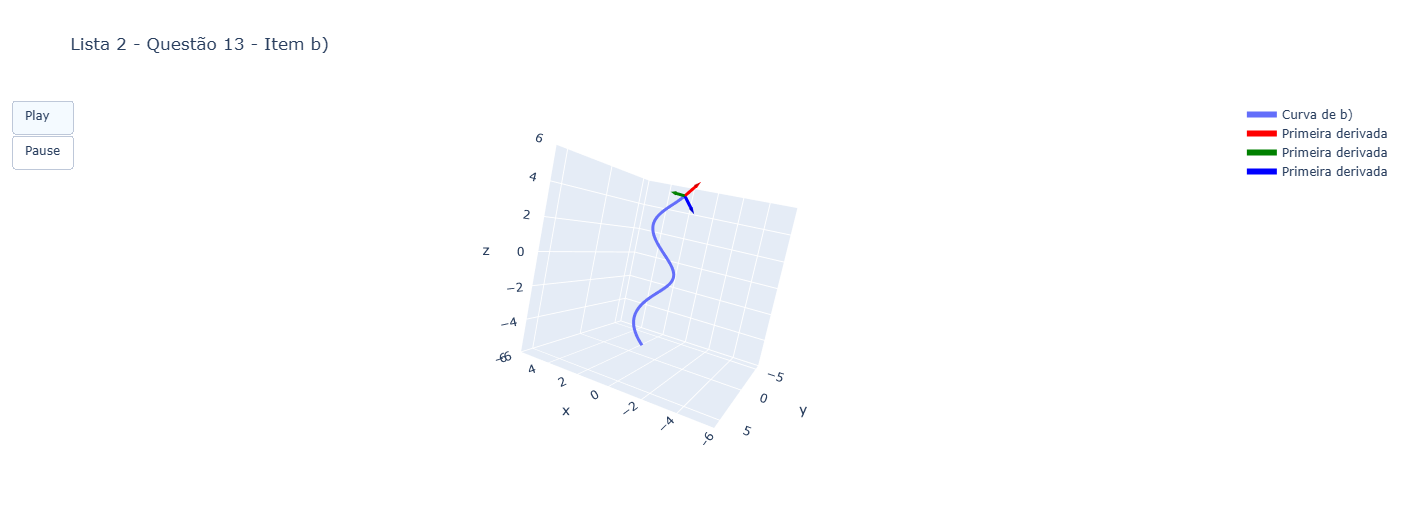
\includegraphics[width=0.5\textwidth]{imagens/lista02/picture_lista02_q13_item02.png}
		\captionof{figure}{Questão 13 - Item b)}
	\end{center}
\end{solucao}

\begin{exercicio}{14}
	Calcule a curvatura e a torção das seguintes curvas:
	\begin{enumerate}[label=\alph*)]
		\item $\alpha(t)=(t, t^2, t^3)$, $t\in \mathbb{R}$
		\item $\beta(t)=(\cos(t), \sin(t), t)$, $t\in \mathbb{R}$
	\end{enumerate}
\end{exercicio}

\begin{solucao}
	\begin{enumerate}[label=\alph*)]
		\item 
		Calculando as derivas de primeira, segunda e terceira ordem, obtemos:
		\begin{itemize}
			\item $\alpha'(t)=(1,2t,3t^2)$
			\item $\alpha''(t)=(0,2,6t)$
			\item $\alpha'''(t)=(0,0,6)$
		\end{itemize}
		
		Pelas fórmulas da curvatura $k$ e torção $\tau$, temos
		
		\begin{itemize}
			\item 
			$k_\alpha(t)=\frac{\|\alpha'(t) \wedge \alpha''(t)\|}{\|\alpha'(t)\|^3}$
			
			$\Rightarrow k_\alpha(t)=\frac{\|(\det\big[ (2t,3t^2), (2,6t)\big],-\det\big[(1,3t^2),(0,6t)\big], \det\big[ (1,2t), (0,2)\big])\|}{(1+4t^2+9t^4)^{\frac{3}{2}}}$
			
			$\Rightarrow k_\alpha(t)=\frac{\|(6t^2,6t,2)\|}{(1+4t^2+9t^4)^{\frac{3}{2}}}=\frac{2(9t^4+9t^2+1)^{\frac{1}{2}}}{(1+4t^2+9t^4)^{\frac{3}{2}}}$
			
			\item $\tau_\alpha(t)=\frac{\left\langle \alpha'(t) \wedge \alpha''(t), \, \alpha'''(t) \right\rangle}{\left\|\alpha'(t) \wedge \alpha''(t)\right\|^2}=\frac{\left\langle 2(3t^2,3t,1), \, (0,0,6) \right\rangle}{2^2\cdot (9t^4+9t^2+1)}=\frac{12}{4\cdot(9t^4+9t^2+1)}$
			
			$\Rightarrow \tau_\alpha(t)=\frac{3}{9t^4+9t^2+1}$
		\end{itemize}
		
		\item 
		Calculando as derivas de primeira, segunda e terceira ordem, obtemos:
		\begin{itemize}
			\item $\beta'(t)=(-\sin(t),\cos(t),1)$
			\item $\beta''(t)=(-\cos(t),-\sin(t),0)$
			\item $\beta'''(t)=(\sin(t),-\cos(t),0)$
		\end{itemize}
		
		Pelas fórmulas da curvatura $k$ e torção $\tau$, temos
		
		\begin{itemize}
			\item $k_\beta(t)=\frac{\|\beta'(t) \wedge \beta''(t)\|}{\|\beta'(t)\|^3}$
			
			{\scriptsize
				$k_\beta(t)=\frac{\|(\det \tiny\begin{pmatrix} \cos(t)&-\sin(t)\\1 &0 \end{pmatrix},-\det\tiny\begin{pmatrix} -\sin(t)&-\cos(t)\\1 &0 \end{pmatrix}, \det\tiny\begin{pmatrix} -\sin(t)&-\cos(t)\\\cos(t) &-\sin(t) \end{pmatrix})\|}{((-\sin(t)^2+\cos^2(t)+1)^{\frac{3}{2}}}$
			}
			
			$k_\beta(t)=\frac{\|(\sin(t), -\cos(t), \sin^2(t)+\cos^2(t))\|}{2^{\frac{3}{2}}}=\frac{\|(\sin(t), -\cos(t), 1)\|}{2^\frac{3}{2}}$
			
			$k_\beta(t)=\frac{\sqrt{\sin^2(t)+(-\cos(t))^2+1}}{2^{\frac{3}{2}}}=\frac{2^{\frac{1}{2}}}{2^{\frac{3}{2}}}=2^{-1}$
			\item $\tau_\beta(t)=\frac{\left\langle \beta'(t) \wedge \beta''(t), \, \beta'''(t) \right\rangle}{\left\|\beta'(t) \wedge \beta''(t)\right\|^2}=\frac{\left\langle (\sin(t),-\cos(t), 1),\, (\sin(t),-\cos(t),0) \right\rangle}{ \sin^2(t)+(-\cos(t))^2+1}$
			
			$\tau_\beta{(t)=\frac{\sin^2(t)+\cos^2(t)}{2}}=\frac{1}{2}$
		\end{itemize}
	\end{enumerate}
\end{solucao}

\end{document}
